Emotional Execution Tree is a connected acyclic graph $G(V,E)$ with $|V|$ vertexes and $|E|$ edges. The root and non-leaf nodes could be of either \textit{parallel} or \textit{sequential} type, which represent the type of actions that would be executed by the system. Sequential nodes execute one branch after the other. Once all the branches have been executed, asequential node notifies its predecessor to continue with the execution of other branches. The parallel node executes all the branches at the same time. This type of node offers two levels of synchronization: action and emotion. The action level synchronization enables the possibility to stop all the branches once the main branch has completed its execution. This main branch is established in the action message. On the other hand, the emotion level synchronization updates to a new emotional parameter of all the branches once the main branch updates to a new emotional parameter. %TODO The previous sentence is not clear. I cannot understando so I cannot fix it. What does it mean that updates to a parameter?
In both cases, any update or finish message will be ignored if the branch is not principal. These two levels of synchronization create four sub-types of parallel nodes: (i) action and emotion synchronous, (ii) action synchronous and emotion asynchronous, (iii) action asynchronous and emotion synchronous, or (iv) action and emotion asynchronous. 
 
Finally, leaf nodes are only simple action nodes that have been implemented in the system. Any node can belong to one of two levels: principal or secondary. If a node is principal, it will notify its predecessor about the messages that it has received, while the secondary node cannot propagate any message to its predecessor. This enables the possibility to have actions that have priority over others. To exemplify this, let us consider the sequence of actions depicted in Figure~\ref{fig:sequence_actions}. The Emotional Execution Tree for this sequence would be like the one presented in Figure~\ref{fig:emotional_enrichment}.

\begin{figure}
	\centering
	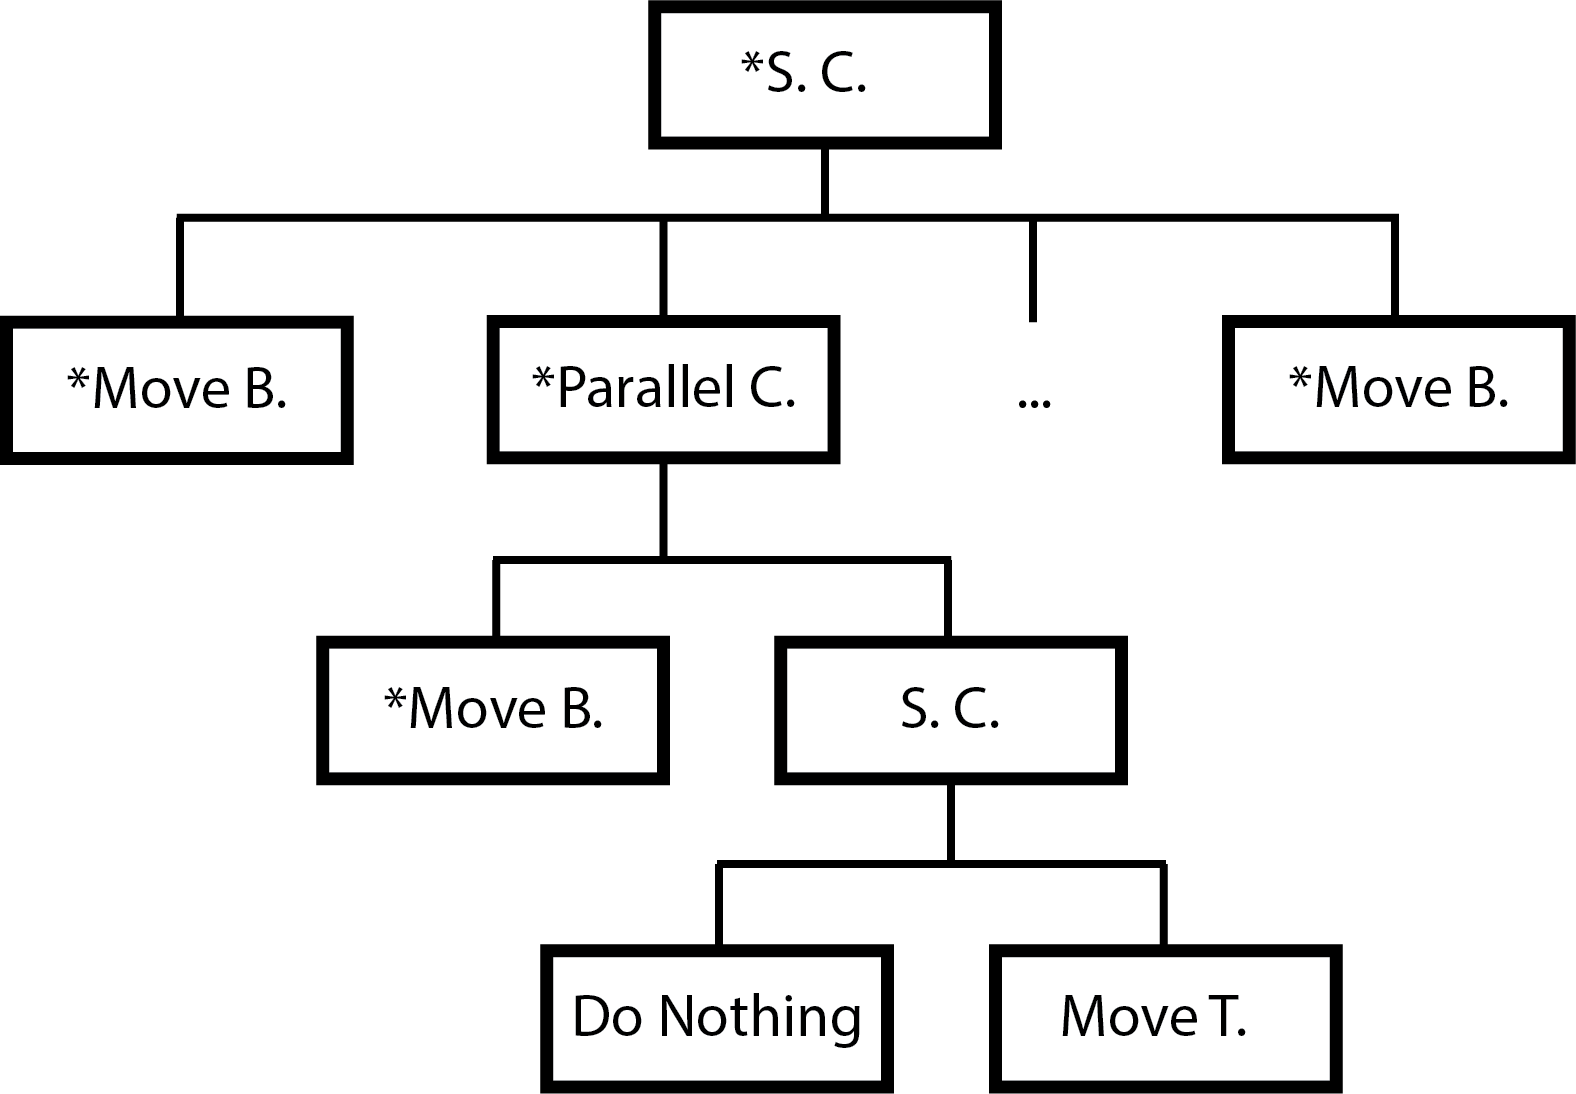
\includegraphics[width=0.45\textwidth]{./Images/Representation.png}
	\caption{Emotional Execution Tree for the sequence of actions depicted in Figure~\ref{fig:sequence_actions}. The $*$ symbol denotes principal nodes. $S$ represents sequential.}
	\label{fig:emotional_enrichment}
\end{figure}

\subsection{Formalization of Simple and Compound Actions}
Formalizing simple and compound actions enables the generation of a system to design them and verify if they are described correctly. Simple actions ($SA$) could be seen as functions that map a set of parameters $p^{pl}_{i} \in P$ to specific platform ($pl$) movements ($m^{pl}_{j}\in M^{pl}$) in the set of movements for that platform ($m^{pl}_{j} =sa^{pl}(\lbrace p^{pl}_{i} \rbrace)$). Each $sa^{pl}$ could have different implementations due to different reasons such as: platform's configuration, action's goal, how the mapping from inputs to outputs are done, among others. 
In our case, we consider that two actions are different if $(\forall sa_{i}, sa_{j} \in SA, \forall q, t \in PL | Param( sa_{i}^q ) \neq Param( sa_{j}^t )\Rightarrow sa_{i}^q \neq sa_{j}^t)$, 
where $PL$ is the set of all the possible platforms, $Param(\cdot)$ returns the set of parameters that are input of the $sa$ (e.g., $vel$,$pitch$,$text$). 
On the other hand, we will consider two actions as equivalents if $(\forall sa_{i}, sa_{j} \in SA , \forall q, t \in PL | Param( sa_{i}^q ) = Param(sa_{j}^t ) \wedge Obj(sa_{i}^q) = Obj(sa_{j}^t) \Rightarrow sa_{i}^q \equiv sa_{j}^t)$,  
where $Obj(\cdot)$ returns the set of objectives that are intended to be achieved by a given action. This $SA$ equivalence allows us to avoid the specification of all the platforms for all the actions that share the same objective and hide leaf nodes that do not give relevant information to understand the emotional tree.

With this $SA$ definition, it is now possible to define emotion enrichment as $ (\forall sa \in SA, \forall e \in E, \exists \; en$ $|$ $en=Enrichment(sa,e,Param(sa), Intensity(e)))$, where $Intensity(\cdot)$ returns the intensity of a given emotion, $E$ is the set of emotions, and $en$ can be the same $sa$, but with the parameters modified in order to convey the desired emotion $e$, or even a set of $sa$ with modified parameters. This definition goes along with the idea that new $sa$ could be added to convey a specific emotion. In addition, the $Enrichment(\cdot)$ function has the following properties:
\begin{itemize}
	\item $(\forall sa_{i},sa_{j} \in SA, \forall e \in E$ $|$ $sa_{i} \equiv sa_{j} \Rightarrow Enrichment(sa_{i},e,...) \equiv Enrichment(sa_{j},e,...))$
	\item $(\forall sa_{i},sa_{j} \in SA, \forall e \in E$ $|$ $(sa_{i} \not\equiv sa_{j}) \Rightarrow Enrichment(sa_{i},e,...) \not \equiv Enrichment(sa_{j},e,...))$
\end{itemize}

The concept of compound action ($CA$) is defined as $g = ca(\{p_{i}\})$, where $(p_{i} \in Param(sa))$, $(sa \subseteq SA)$, $(g \in EXT)$.
